\documentclass{article}
%\usepackage[utf8]{inputenc}
\usepackage{fullpage}
\usepackage{amsfonts}
\usepackage{amsmath}
\usepackage{amssymb}
\usepackage{subfigure}
\usepackage{tabularx}
\usepackage{url}
\usepackage{times}  % DO NOT CHANGE THIS
\usepackage{helvet}  % DO NOT CHANGE THIS
\usepackage{courier}  % DO NOT CHANGE THIS
\usepackage[hyphens]{url}  % DO NOT CHANGE THIS
\usepackage{subcaption}
\usepackage{graphicx}
\urlstyle{rm} % DO NOT CHANGE THIS
\def\UrlFont{\rm}  % DO NOT CHANGE THIS
\usepackage{natbib}  % DO NOT CHANGE THIS AND DO NOT ADD ANY OPTIONS TO IT
\usepackage{caption} % DO NOT CHANGE THIS AND DO NOT ADD ANY OPTIONS TO IT
\usepackage{algorithm}
\usepackage{algorithmic}
\usepackage[usenames,dvipsnames]{xcolor}
\usepackage{verbatim}
\newcommand{\eqr}{\ensuremath{P(L_{\epsilon}(Q(D))}}
%\usepackage[utf8]{inputenc}
\usepackage{fullpage}
\usepackage{amsfonts}
\usepackage{amsmath}
\usepackage{amssymb}
\usepackage{subfigure}
\usepackage{tabularx}
\usepackage{url}
\usepackage{times}  % DO NOT CHANGE THIS
\usepackage{helvet}  % DO NOT CHANGE THIS
\usepackage{courier}  % DO NOT CHANGE THIS
%\usepackage[hyphens]{url}  % DO NOT CHANGE THIS
\usepackage{subcaption}
\usepackage{graphicx}
\urlstyle{rm} % DO NOT CHANGE THIS
\def\UrlFont{\rm}  % DO NOT CHANGE THIS
\usepackage{natbib}  % DO NOT CHANGE THIS AND DO NOT ADD ANY OPTIONS TO IT
\usepackage{caption} % DO NOT CHANGE THIS AND DO NOT ADD ANY OPTIONS TO IT
\usepackage{algorithm}
\usepackage{algorithmic}
%\usepackage[usenames,dvipsnames]{xcolor}
\usepackage{verbatim}
\newcommand{\eqr}{\ensuremath{P(L_{\epsilon}(Q(D))}}\begin{document}

%\title{A Risk-Aware Paradigm for Privacy-Preserving Machine Learning}
%\author{Murat Kantarcioglu \thanks{ muratk@utdallas.edu, University of Texas at Dallas and Harvard University}}
%\date{}
%\maketitle


\begin{abstract} 
Over the years, the increasing use of personal data for training machine learning models raises several privacy concerns,  %many privacy challenges have been identified in the context of the data science, machine learning (ML) model training and deployment, ranging from 
such as membership inference attacks (i.e., detecting whether a given individual is in the training data) and sensitive attribute inference attacks (i.e., predicting some sensitive information about users based on the disclosed ML model).
Although privacy solutions have emerged to address individual challenges, there is not a silver-bullet solution for all privacy problems.
%Although specific privacy solutions have emerged to address such challenges,  
%{\it any single} solution often does not result in a satisfactory outcome.

In this opinion paper, we argue that %any single privacy solution  
%could not solve all 
%there is not a silver-bullet solution for all the privacy problems, and 
to develop a complete solution to a multitude of privacy challenges, 
we need a privacy-risk aware paradigm  %where different tools and techniques are integrated using realistic privacy threats.
where tools and techniques targeting individual realistic privacy threats are employed simultaneously to complement each other. 
To achieve this goal, we propose a generic privacy framework to reason about the optimal combination of existing privacy tools under the set of given attack models and discuss how the proposed framework could be applied in practice.
\end{abstract}

\section{Introduction}
Sharing data while preserving individual privacy has emerged as a fundamental challenge in the age of big data and the prevalent use of machine learning (ML) models. While many privacy-preserving solutions/techniques have been developed, it is not always clear how to strike a balance %achieve the right balance 
between utility and privacy. We postulate that this fundamental problem cannot be solved with just one privacy definition/tool alone. 

Different ML challenges may require the integration of the existing and new tools to achieve the desired utility and privacy balance under different privacy definitions. We believe that such scenarios could be addressed by moving into a privacy-risk estimation paradigm that can be used to analyze the privacy risks and the utility provided by different privacy-preserving tools and techniques under different realistic attack models and existing regulatory frameworks. 

Such a threat aware risk assessment is already in use in several domains. For example, to measure door lock security, the American National Standards Institute defines a series of tests that simulate real life attacks against door locks. Examples of these attacks include the application of force (e.g., someone who is trying multiple kicks to %kick the door down
knock the door open),  
and a battery of lock picking tests. The lock is assigned a grade based on its success against these types of likely attacks. \footnote{\url{https://blog.ansi.org/2020/01/ansi-grade-levels-bhma-locks-hardware-tests/\#gref}. Please note, ANSI is not NIST.} Clearly, the door locks can be picked by expert locksmiths given enough time. In addition, they can be easily opened by deploying explosives and significant brute force. The existing vulnerabilities to these other attacks are considered natural and different mechanisms (e.g., alarm systems) are used to protect against these other types of attacks. 

Similarly, most ATM networks use a four digit pin for money withdrawals instead of a 6 digit pin for better usability %reasons 
(harder to memorize a 6 digit pin). To limit risks, usually there are limits on how much one person can withdraw in a given day and how many times one can enter the pin before the ATM card is disabled.  Such an approach could be seen as a practical risk-aware solution against reasonable threats (e.g., someone randomly trying the ATM card) that balances utility/usability %(e.g., using only a 4 digit pin) 
and risks. 

In many domains, risk-based data sharing ideas have been applied for many years without rigorous %rigorously analyzing 
analysis of the privacy risks.  One example is the airline passenger wait lists used at many US airports. %In figure 
Figure~\ref{fig:airline} shows a first class upgrade list for an example flight. The passengers on a given flight can use such lists to check whether they are upgraded to the first class or whether they can stand by for the upcoming flight. To reduce privacy risks, only the first character of the given name and the first three characters of the last name are used on these lists. Furthermore, to access these waitlists, you should be at a specific airport near the flight gate and/or checked in via the airline app. Therefore, a combination of access control rules (e.g., only certain people can access to given waitlist data) and simple data sanitization techniques (e.g., redacting full names) provides reasonable protection against certain threats. 
%Yan: I'm not sure how the followng example can support the previous claim of providing reasonable protection.
%MK: Tried to clarify it now.
Clearly, above approach for disclosing passenger wait list information could be attacked under certain scenarios. For example, if the attacker is at the airport and knows a certain targeted individual is traveling that day, the attacker can find which flight that person is on. On the other hand, using publicly available data (e.g., the voter registration list available for Texas or online twitter information) thousands of names will match a given initial. To our knowledge, this information had not been successfully re-identified on a large scale. Our own back-of-the-envelope calculations show that using just the online information such as voter registration lists, the probability of re-identifying a random individual is very low. Hence, under a reasonable threat model (e.g., only using publicly available information and not waiting at the airport to identify an individual), the privacy risk for this sharing is quite limited. Furthermore, combining the data redaction approach with an access control scheme (e.g., you need to be at the airport to launch an attack) makes the potential privacy attacks less likely.


\begin{figure}[!htb]
 \centering
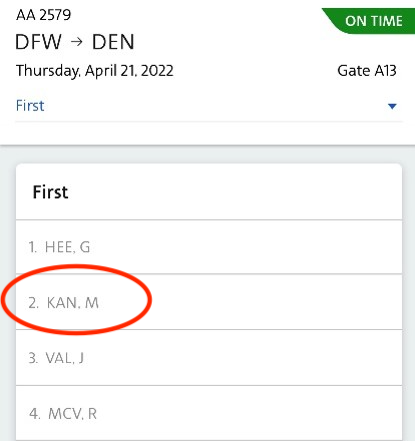
\includegraphics[height=5cm]{letters/airline.png}
 \caption{Risk-based Data Sharing: Airline Wait List. Red circled individual is the author.}
 \label{fig:airline}
\end{figure}


To establish a risk-aware privacy preserving ML framework based on ML use cases, we need to start by understanding utility goals, existing and upcoming attack techniques, potential attacker incentives to launch the attacks, potential attack success under the integration of different privacy-preserving technologies, and the impact of the chosen privacy parameters to get the desired utility and privacy trade-off. For example, for sharing individual level COVID-19 data to build an ML model, we may need to understand how such data could be used to launch re-identification attacks under different data sanitization models and attacker background knowledge \cite{BrownYXYWGKM22}. In addition, we need to understand how different privacy tools and models impact data utility. For example, for building ML models that are predicting pandemic progression for different race groups, preserving race information may provide more utility than releasing more granular age information.  

The above example suggests that different use cases need to be treated 
with realistic privacy attack models, attacker background information, utility goals, acceptable privacy risks, and then reason about the privacy risk vs utility trade-offs under different privacy-preserving technology combinations. This also implies that as the technology and threat landscape evolve, we need to re-evaluate the existing privacy risks, privacy definitions, and their evolving utility.  Below, we discuss how this framework could be applied in the context of privacy-preserving machine learning (ML) applications.

\section{Risk-aware Privacy-preserving Machine Learning}
%Over the years, there have been 
In the face of rising privacy attacks against ML models %ranging from 
such as model inversion and membership inference~\cite{evans-diff} attacks, differential privacy has emerged as the main protection against these attacks. Although the differential privacy mechanism~\cite{diffprivacy} provides important protections, empirical evaluations have shown that, in many cases, the $\epsilon$ value (one of the parameters needed for tuning the added noise) required for protecting against a certain attack (e.g., model inversion attack) %where a sensitive attribute is predicted given the ML model) 
may significantly %totally 
harm the utility of the ML model \cite{Fredrikson:2015}. Therefore, finding the privacy parameter (e.g., $\epsilon$ in differential privacy) that provides desired utility and adequate protection against attacks may not always be feasible. 

Our proposed risk-based privacy framework could be used to incorporate data sanitization based pre-processing (e.g., sanitizing data before it is used by a differentially private learning mechanism) and post-processing  techniques (e.g, providing a wrapper for a given classifier to reduce model inversion attack success) combined with carefully selected privacy parameters (e.g. $\epsilon$ for differential privacy) to exhibit good utility and adequate protection against realistic privacy attacks.  

The above adversarial attack modeling approach implies that we can first pre-process the data using a data sanitization technique $Q \in \mathcal{Q}$ to get a sanitized version $Q(D)$. In this setting, to make the optimization problem solvable, we can specify a suitable set of sanitization options $\mathcal{Q}$. 
%For example, we can replace sensitive information such as birthdates with a sanitized age information before a ML model is built so that a text generation algorithm will not accidentally memorize them. Alternatively, as we discuss in the synthetic data generation setting, some correlated information may be removed to prevent certain attacks.
%For pre-processing techniques, we can leverage sanitization and random data generation approaches. We believe that many of the issues with respect to a model memorizing sensitive information from the data set could be reduced by replacing sensitive data with similar looking sanitized versions. 
For example, a feature in the Covid-19 dataset that is representing the birthday of a given patient could be replaced with two attributes representing the age bracket the patient belongs to (e.g., replacing 01.01.1993 with $\mapsto (25,35)$). For each attribute, different generalization/sanitization options could be used to describe the possible set of sanitizations available (i.e., $\mathcal{Q}$).

Once the sanitized data is created, a differentially private learning algorithm $L$ with an appropriate privacy parameter $\epsilon$ is chosen to learn a model $M$. Later on, this model is post-processed using a post-processing technique $P$ to make sure that certain attacks are not successful. For example, for a deep learning model $M$, additional neural network layers could be added to $M$ and these layers could be fine-tuned using publicly available data (hence, negligible additional privacy risk) to reduce the effectiveness of specific attacks. These possible post-processing architecture space could be leveraged to specify the potential post-processing options $\mathcal{Q}$. 

Similarly, for classification tasks, we can explore whether the output probabilities of a classifier can be modified to reduce model inversion attack success. For example, an overly confident class prediction may help an attacker to better infer a sensitive attribute. For generative machine learning models, we may explore different post-processing models to automatically sanitize potentially sensitive output. For example, we may learn a model $P$ that can detect sensitive data such as a social security number (ssn) predicted by the machine learning model $M$, and redact it automatically. 

The proposed approach leads to an optimization problem (See Equation~\ref{eqn:m}) where we find the optimal combination of $\epsilon, P \in \mathcal{P}, Q \in \mathcal{Q}$ such that we maximize the  model utility (e.g., accuracy) while making sure that privacy risk (e.g., sensitive attribute prediction accuracy) due to an attack $i$ is less than the desired privacy risk limit $\gamma_i$. Depending on the use case, we need to develop define appropriate pre-processing $\mathcal{P}$ and post-processing $\mathcal{Q}$  options for different machine learning tasks against  different types of attacks, and for each attack type $i$ (e.g., membership inference attack), we need to measure the privacy risk  $\mbox{Risk-Attack}_i$. 

\begin{equation}
\begin{aligned}
\max_{\epsilon, P \in \mathcal{P},Q \in \mathcal{Q}} \quad & \mbox{Utility}(\eqr)\\
\textrm{s.t.} \quad & \mbox{Risk-Attack}_1( \eqr ) \leq \gamma_1\\
& ......\\
                    %&\mbox{Risk-Attack}_2( \eqr  ) \leq  \gamma_2\\
                    &\mbox{Risk-Attack}_n(\eqr   )  \leq \gamma_n \\
\end{aligned}
\label{eqn:m}
\end{equation}

%As the above examples suggest many of the existing data sanitization approaches can be combined with differentially private models to learn useful models. 

%That is, a name and surname pair, could be replaced with a realistic random version to hide personally identifiable information. 


\subsection{Example Application: Privacy-preserving Explanation Generation}

In our previous work~\cite{yasmeen-tdsc}, we applied such a risk-aware privacy approach and showed that a differentially private explainable ML model (i.e., a rule set that explains a given ML model) could be post processed (e.g., some rules may be pruned) to achieve better accuracy while being more resistant to model inversion attacks. Similar to previous observations in the literature~\cite{Fredrikson:2015}, a pure differentially private model could not reach the desired protection against model inversion attacks while providing accurate prediction accuracy. Instead, our proposed risk based approach achieved both goals while being differentially private using a higher $\epsilon$ value. Our approach is not intended to replace differential privacy. In this approach, we use differential privacy with larger $\epsilon$ combined with our privacy-aware data pruning technique to preserve both utility and privacy. 

Our strategy proceeds as follows:
\begin{enumerate}
\item We build a differentially private machine learning model;
\item The predictions produced by the machine learning model are used as an input to a rule-based explanation model. Therefore, the rules are generated from the predictions produced by differentially private learning models; 
\item Our privacy risk estimator named $\alpha$-violation is applied to prevent  model inversion attacks.
\item Using the estimated risks and potential utility, some rules that are too risky are pruned.
\end{enumerate}
The complete strategy for combining differential privacy  with our privacy risk estimator is given in Figure~\ref{fig:DP_alpha}.

Our results indicate that such an approach could use a much higher $\epsilon$ value (i.e., much less noise) to increase the utility of the generated rules while being resistant to model inversion attacks.

\begin{figure}[!htb]
 \centering
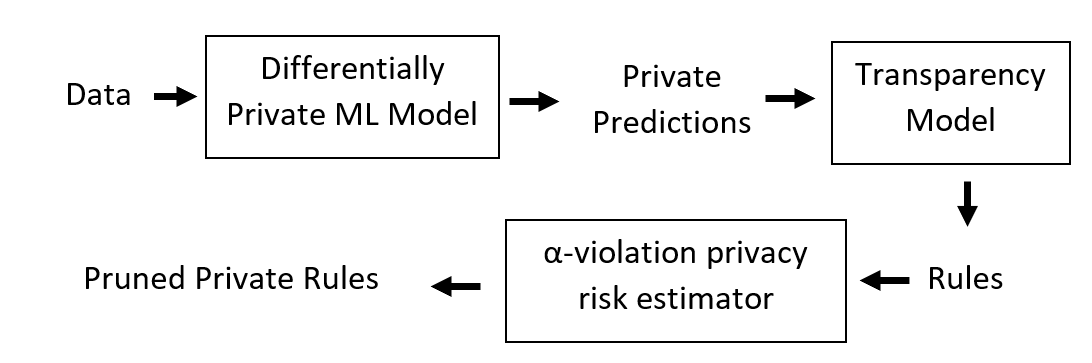
\includegraphics[height=3cm]{letters/PPModel.PNG}
 \caption{The steps for combining differential privacy  with privacy risk estimator.}
 \label{fig:DP_alpha}
\end{figure}


\section{Future Trajectories and Conclusions}
In this opinion paper, we just sketched the basic outline of the proposed risk-aware privacy framework where different data privacy tools can be combined to prevent realistic attacks.

One important implication for the proposed framework is that we need to understand the attacks and the attacker capabilities well enough to come up with realistic threat models.
Errors in the threat model may result in solutions that may not preserve the privacy well enough in practice. In addition, as the attacker's capabilities evolve, we may need to revisit the protections provided by the existing privacy solutions. To prevent potential privacy attacks, it may be prudent to have a margin of error in our threat model assessment and evolution. For example, even though it may be hard for an attacker to learn all the training data, we may build our threat model assuming that the attacker has the entire training data available to launch a private attribute inference attack. One important challenge would be to find the realistic threat model that could not be easily invalidated in practice in the near future.  As in the explanation generation example, certain techniques  (e.g., building a differentially private based model before generating rules to prevent certain privacy attacks) could be used to limit the potential negative outcomes. Furthermore, we believe that our framework can be also widely applicable to other types of attacks, from data poisoning \cite{mustafa-aaai2021} to test time evasion attacks. 
%We leave such application as the future work.

\bibliographystyle{plain}
%\bibliography{murat-bib}
\begin{thebibliography}{1}

\bibitem{yasmeen-tdsc}
Yasmeen Alufaisan, Murat Kantarcioglu, and Yan Zhou.
\newblock Robust transparency against model inversion attacks.
\newblock {\em {IEEE} Trans. Dependable Secur. Comput.}, 18(5):2061--2073,
  2021.

\bibitem{BrownYXYWGKM22}
J.~Thomas Brown, Chao Yan, Weiyi Xia, Zhijun Yin, Zhiyu Wan, Aris
  Gkoulalas{-}Divanis, Murat Kantarcioglu, and Bradley~A. Malin.
\newblock Dynamically adjusting case reporting policy to maximize privacy and
  public health utility in the face of a pandemic.
\newblock {\em J. Am. Medical Informatics Assoc.}, 29(5):853--863, 2022.

\bibitem{Fredrikson:2015}
Matt Fredrikson, Somesh Jha, and Thomas Ristenpart.
\newblock Model inversion attacks that exploit confidence information and basic
  countermeasures.
\newblock In {\em Proceedings of the 22Nd ACM SIGSAC Conference on Computer and
  Communications Security}, CCS '15, pages 1322--1333, NY, USA, 2015. ACM.

\bibitem{evans-diff}
Bargav Jayaraman and David Evans.
\newblock Evaluating differentially private machine learning in practice.
\newblock In {\em 28th {USENIX} Security Symposium ({USENIX} Security 19)},
  pages 1895--1912, Santa Clara, CA, August 2019. {USENIX} Association.

\bibitem{diffprivacy}
Frank~D. McSherry.
\newblock Privacy integrated queries: An extensible platform for
  privacy-preserving data analysis.
\newblock SIGMOD, 2009.

\bibitem{mustafa-aaai2021}
Mustafa~Safa {\"{O}}zdayi, Murat Kantarcioglu, and Yulia~R. Gel.
\newblock Defending against backdoors in federated learning with robust
  learning rate.
\newblock In {\em Thirty-Fifth {AAAI} Conference on Artificial Intelligence,
  {AAAI} 2021}, pages 9268--9276. {AAAI} Press, 2021.

\end{thebibliography}


\end{document}
